\documentclass{beamer}
\usepackage{array}


\title{Irrigation Need}
\subtitle{Project Work on Machine Learning and Data Mining M - B2126}
\author{Luca Zaffaroni}
\date{\today}

\begin{document}

%---------------------------------------------------------
\frame{\titlepage}
%---------------------------------------------------------
%=========================================================

\begin{frame}{Dataset description}

\begin{itemize}
\item The Dataset contains features and informations about ground specifics  (such as soil properties and composition, climatic conditions etc...)  with the goal to predict the need for irrigation,

\item The data set for this competition was generated from a deep learning model trained on the Irrigation Prediction dataset. Feature distributions are close to, but not exactly the same, as the original.

\item Files : 'train.csv'
The competition's training set, used for train validation and test (train size=0.8)

\end{itemize}
\end{frame}

\begin{frame}{Evaluations}
The target is divided into three categories, corresponding to the need for irrigation: low-medium-high
\\Evaluation is based on \textbf{balanced accuracy} between the predicted class and observed target.

\end{frame}


%=========================================================
\section{Dataset overview and insights}
%=========================================================

\begin{frame}{Data types}
    \begin{itemize}
        \item Qualitative features
        \begin{itemize}
            \item Nominal(8): (soil type, crop type, crop growth stage, season, irrigation type, water source, region, mulching used)\\
            \item Ordinal (None) \\
        \end{itemize}    
        \item Quantitative features
            \begin{itemize}
                \item Interval (1): (Temperature C\textdegree)\\
                \item Ratio (10): (soil ph, soil moisture, humidity, organic carbon, electrical conductivity, rainfall mm, sunlight hours, wind speed km-h, field area hectare, previous irrigation mm)\\
            \end{itemize}
        \item Target (irrigation need) \to Nominal
    \end{itemize}
\end{frame}
%=========================================================
\begin{frame}{Feature distributions}
\begin{figure}

    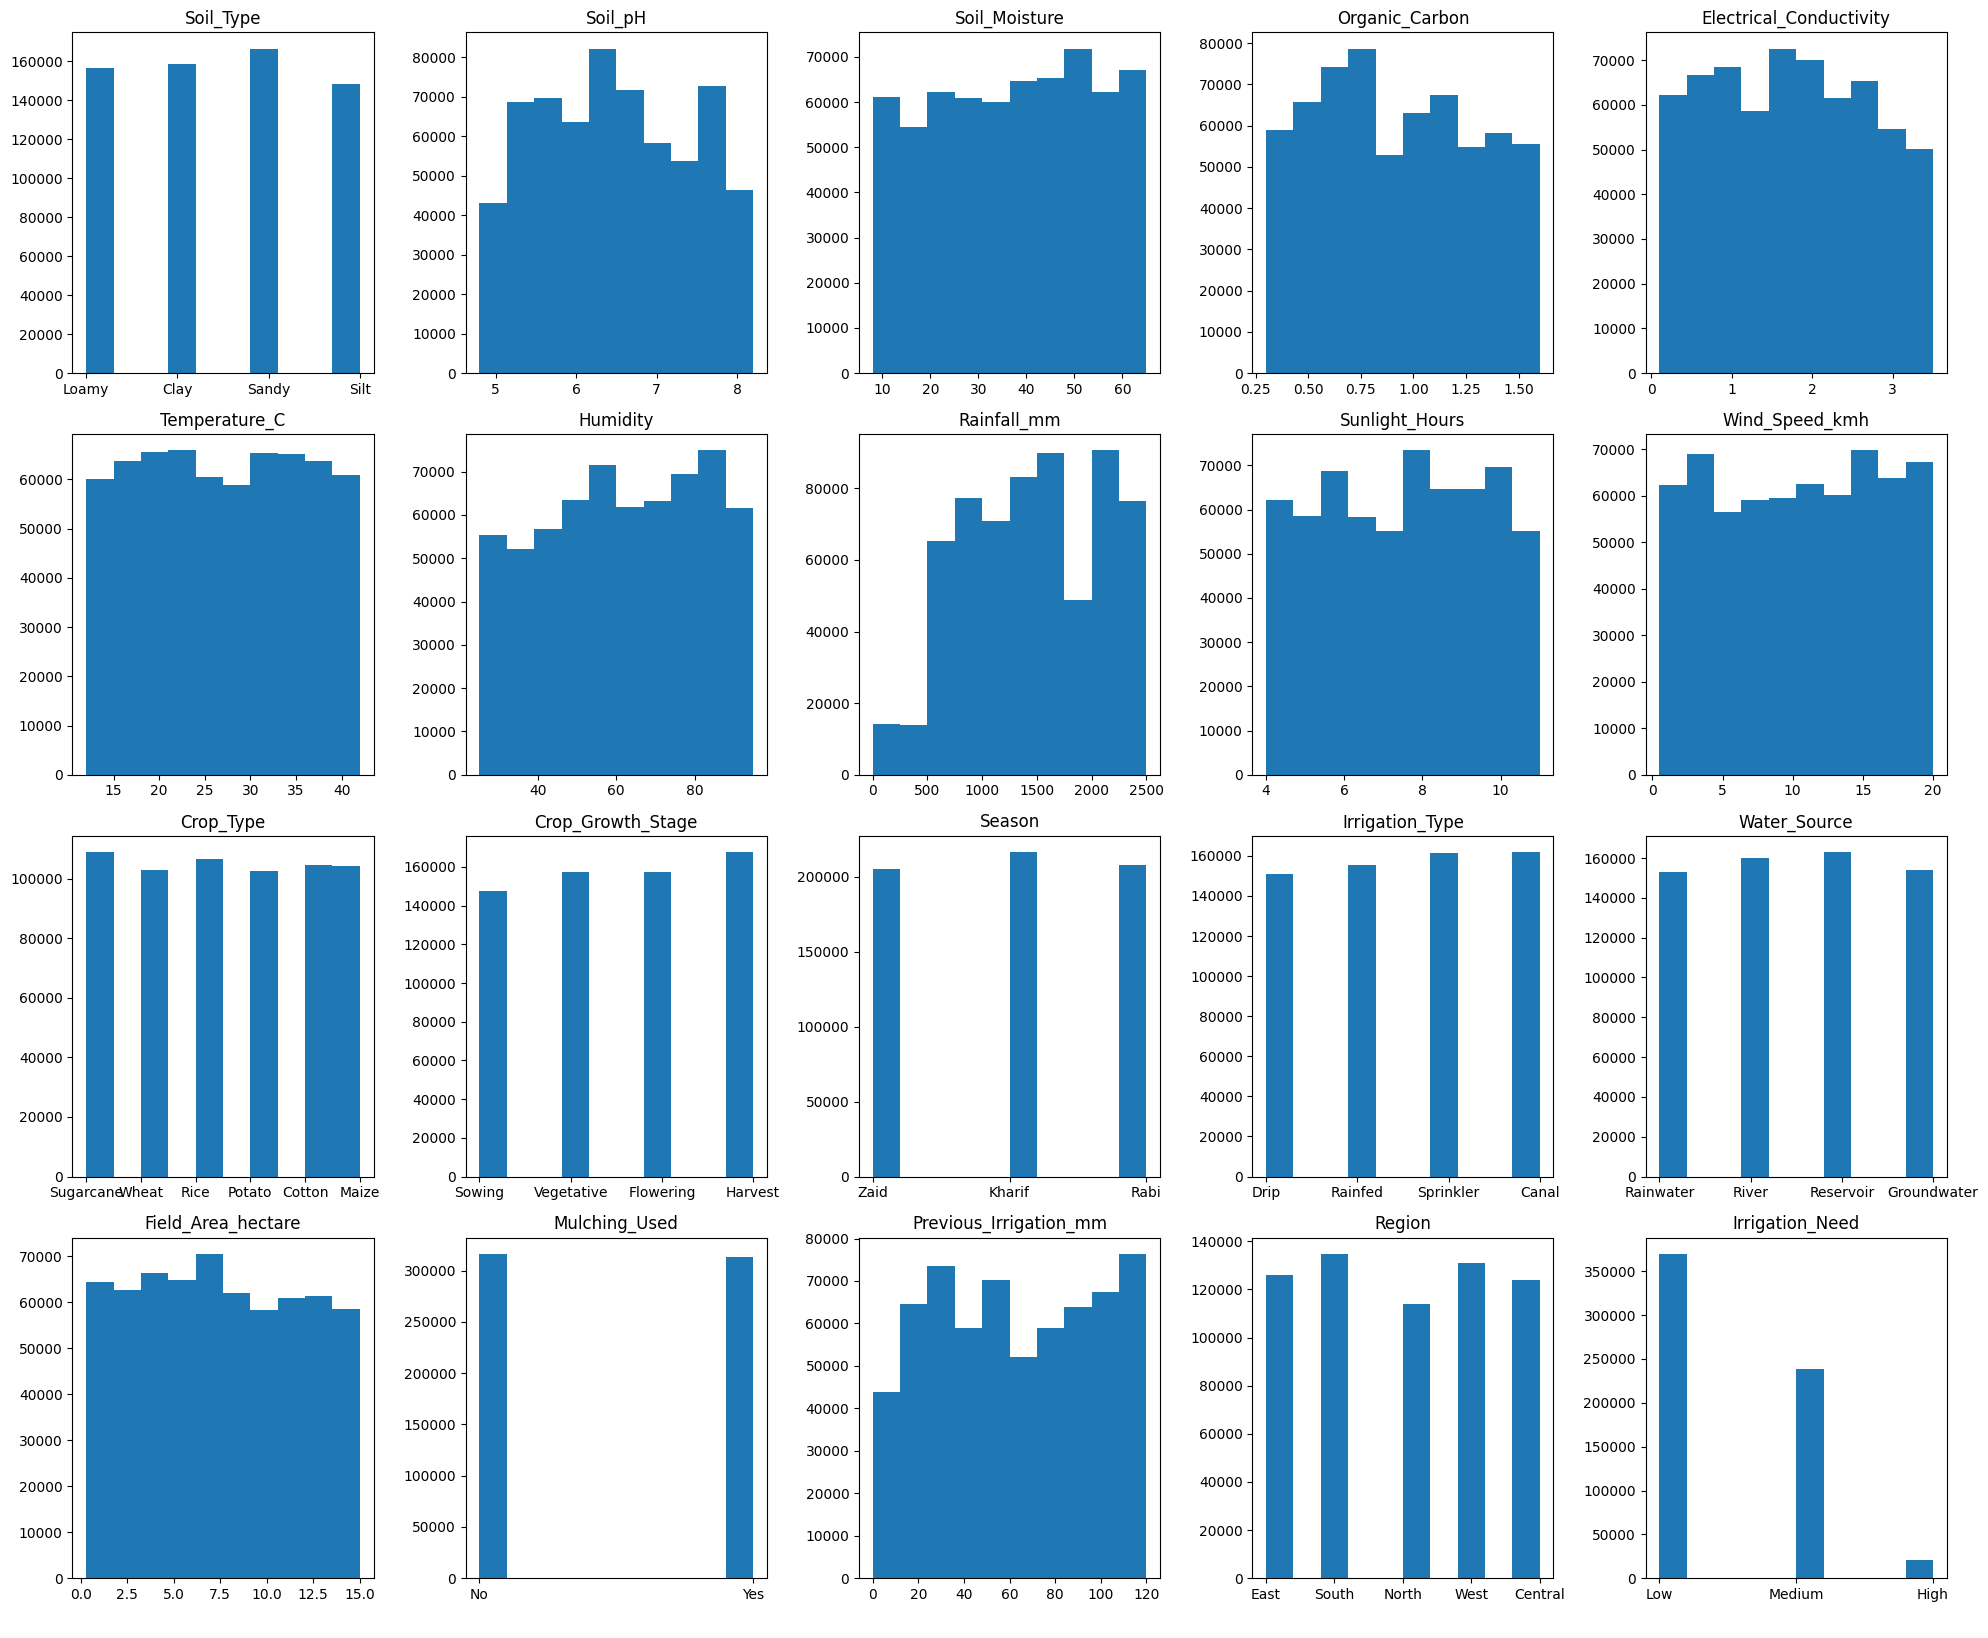
\includegraphics[width=0.45\linewidth]{features_distributions.png}

    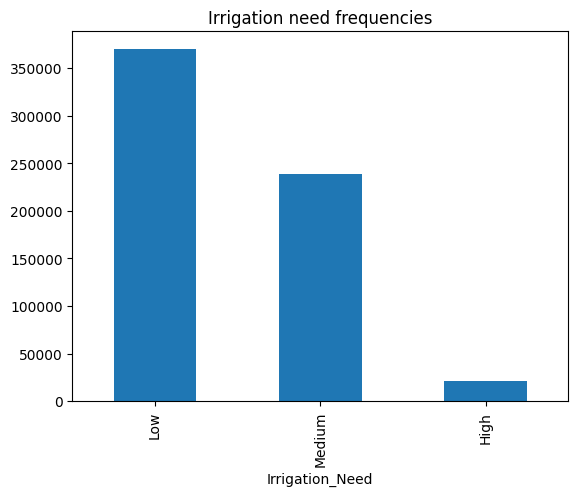
\includegraphics[width=0.25\linewidth]{target_frequencies.png}

    \caption{Features and target distributions: with the exception of soil pH and rainfall (mm), all features show uniform distributions.}
    \label{fig:feature_distributions}
\end{figure}
\end{frame}
%=========================================================
\begin{frame}  
    \begin{figure}
            \centering
            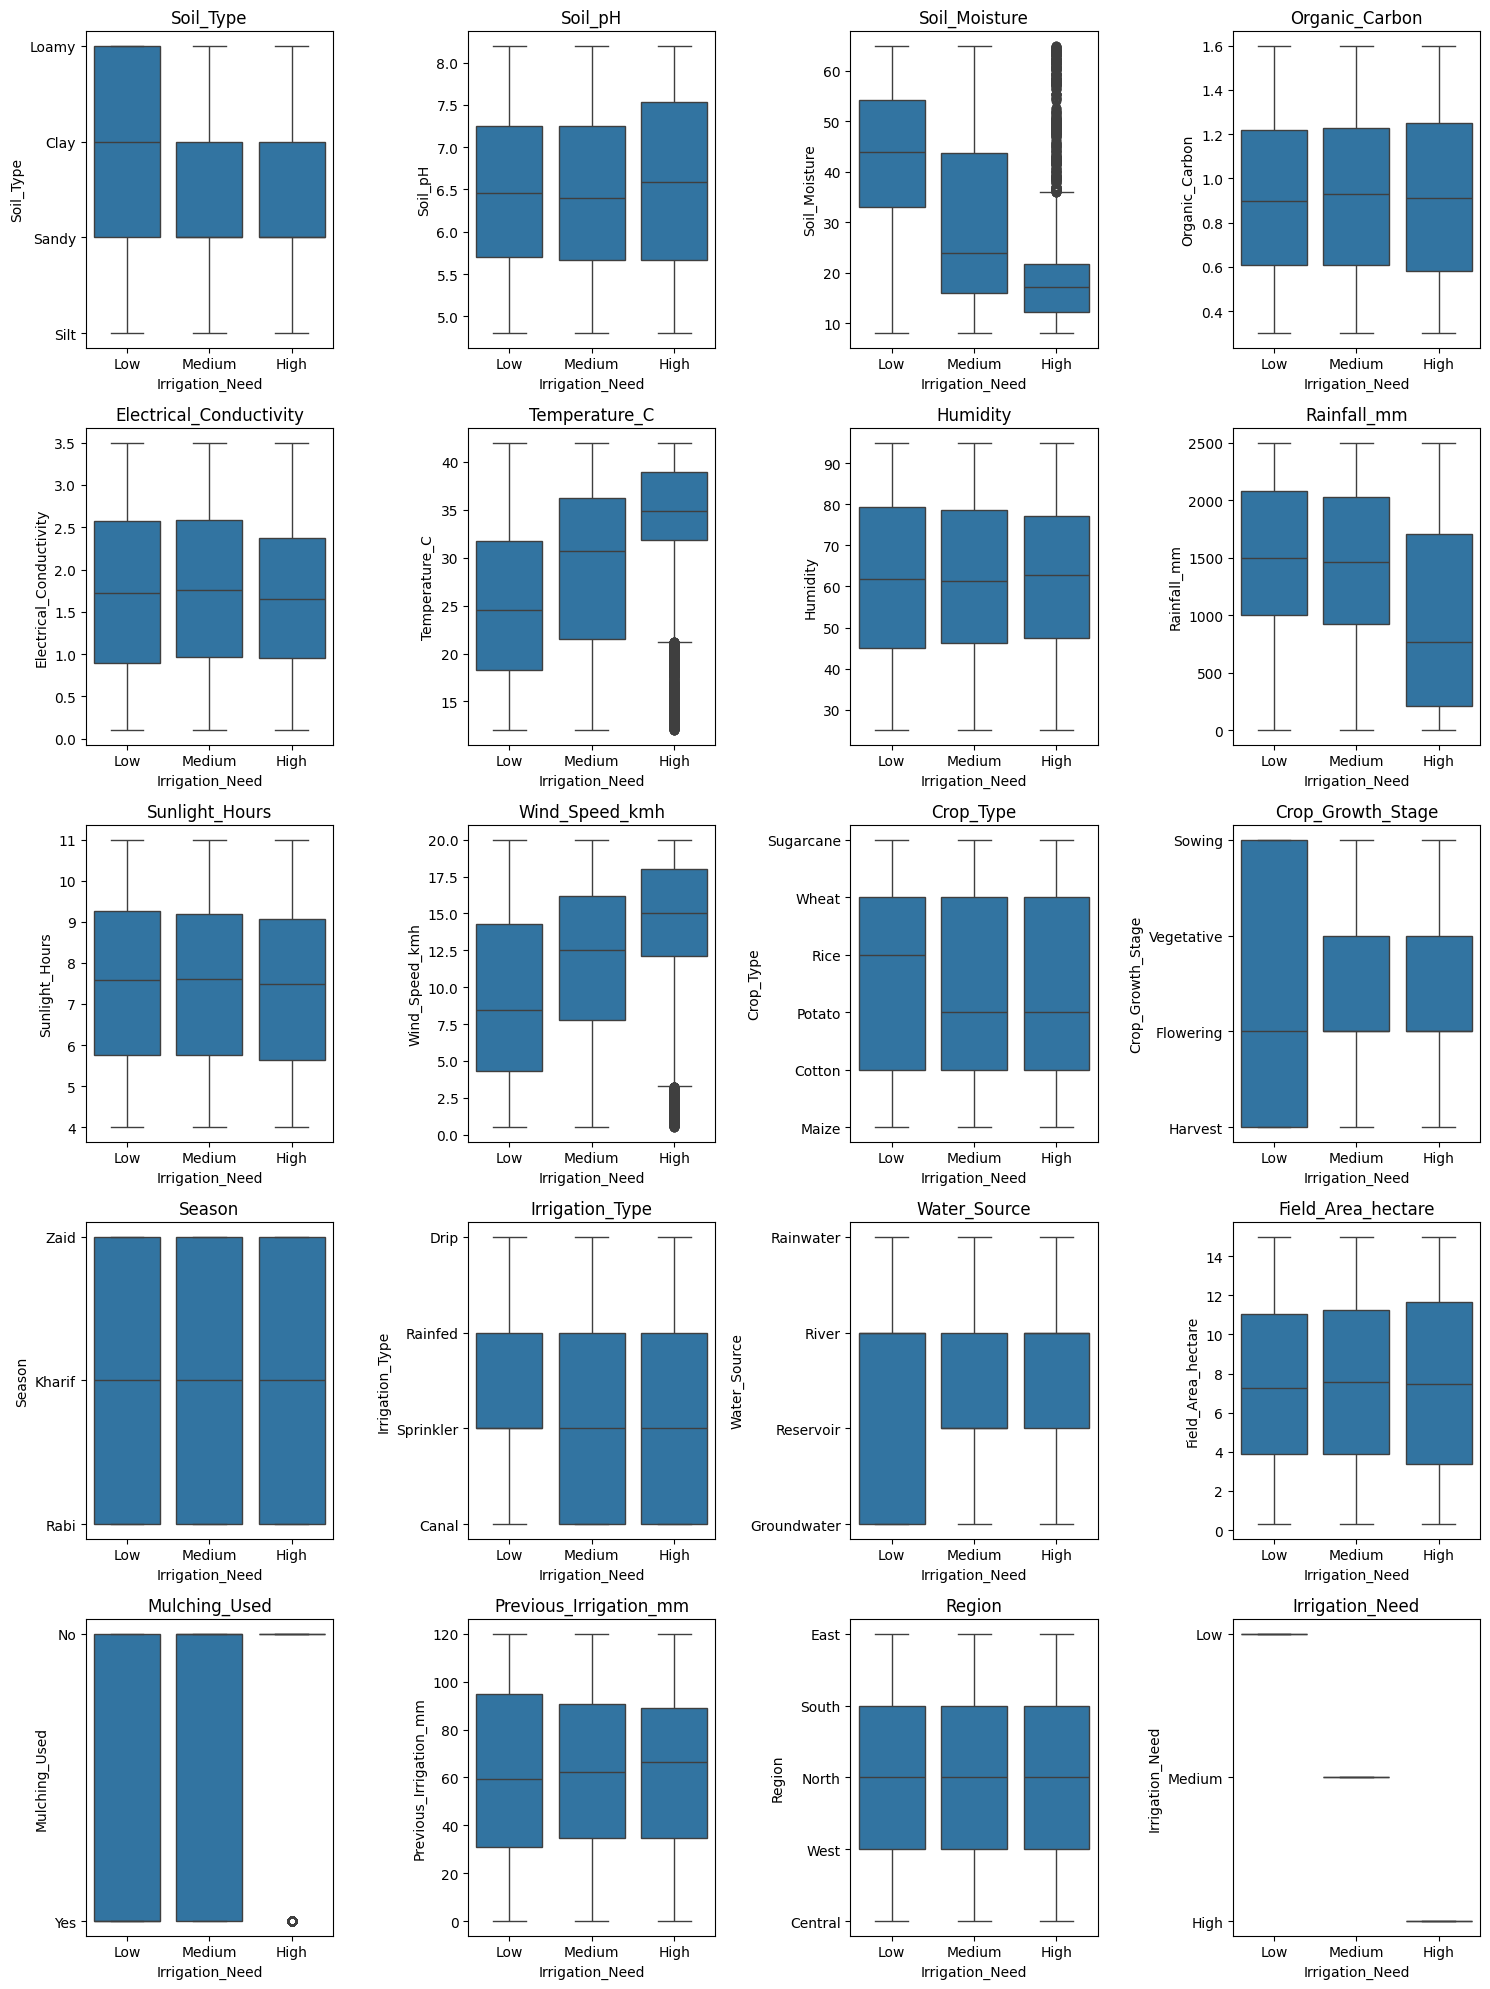
\includegraphics[width=0.40\textwidth]{boxplots.png}
            \caption{Boxplots show how the target value "High" is critical, being the only value with distributions outside the whiskers with lots of outliers}
            \label{fig:placeholder}
        \end{figure}
\end{frame}
%=========================================================
\begin{frame}{More insights...}
    \paragraph{It's worth noticing the imbalance between the already mentioned target class 'High' with respect to the others classes\\ Other important informations can be obtained with a dataframe inspection via pandas API such as:\\
    - df.sample(n)\\
    - df.info()\\
    - df.describe()\\
    
    Our dataset has 630000 entries, 0 to 629999 and 20 columns.\\ The dtypes are: float64(11), object(9) \\
    Memory usage: 100.9+ MB \\
    Finally, our dataset has no null-values.\\}
\end{frame}
%=========================================================
\section{Feature selection}
%=========================================================

\begin{frame}{Methods}
Different possibilities..
\begin{itemize}
    \item PCA
    \item SelectKBest
    \item Other methods (Leave-One-Feature-Out)
\end{itemize}
...but same results..
\end{frame}

\begin{frame}{}
\begin{figure}
    \centering
    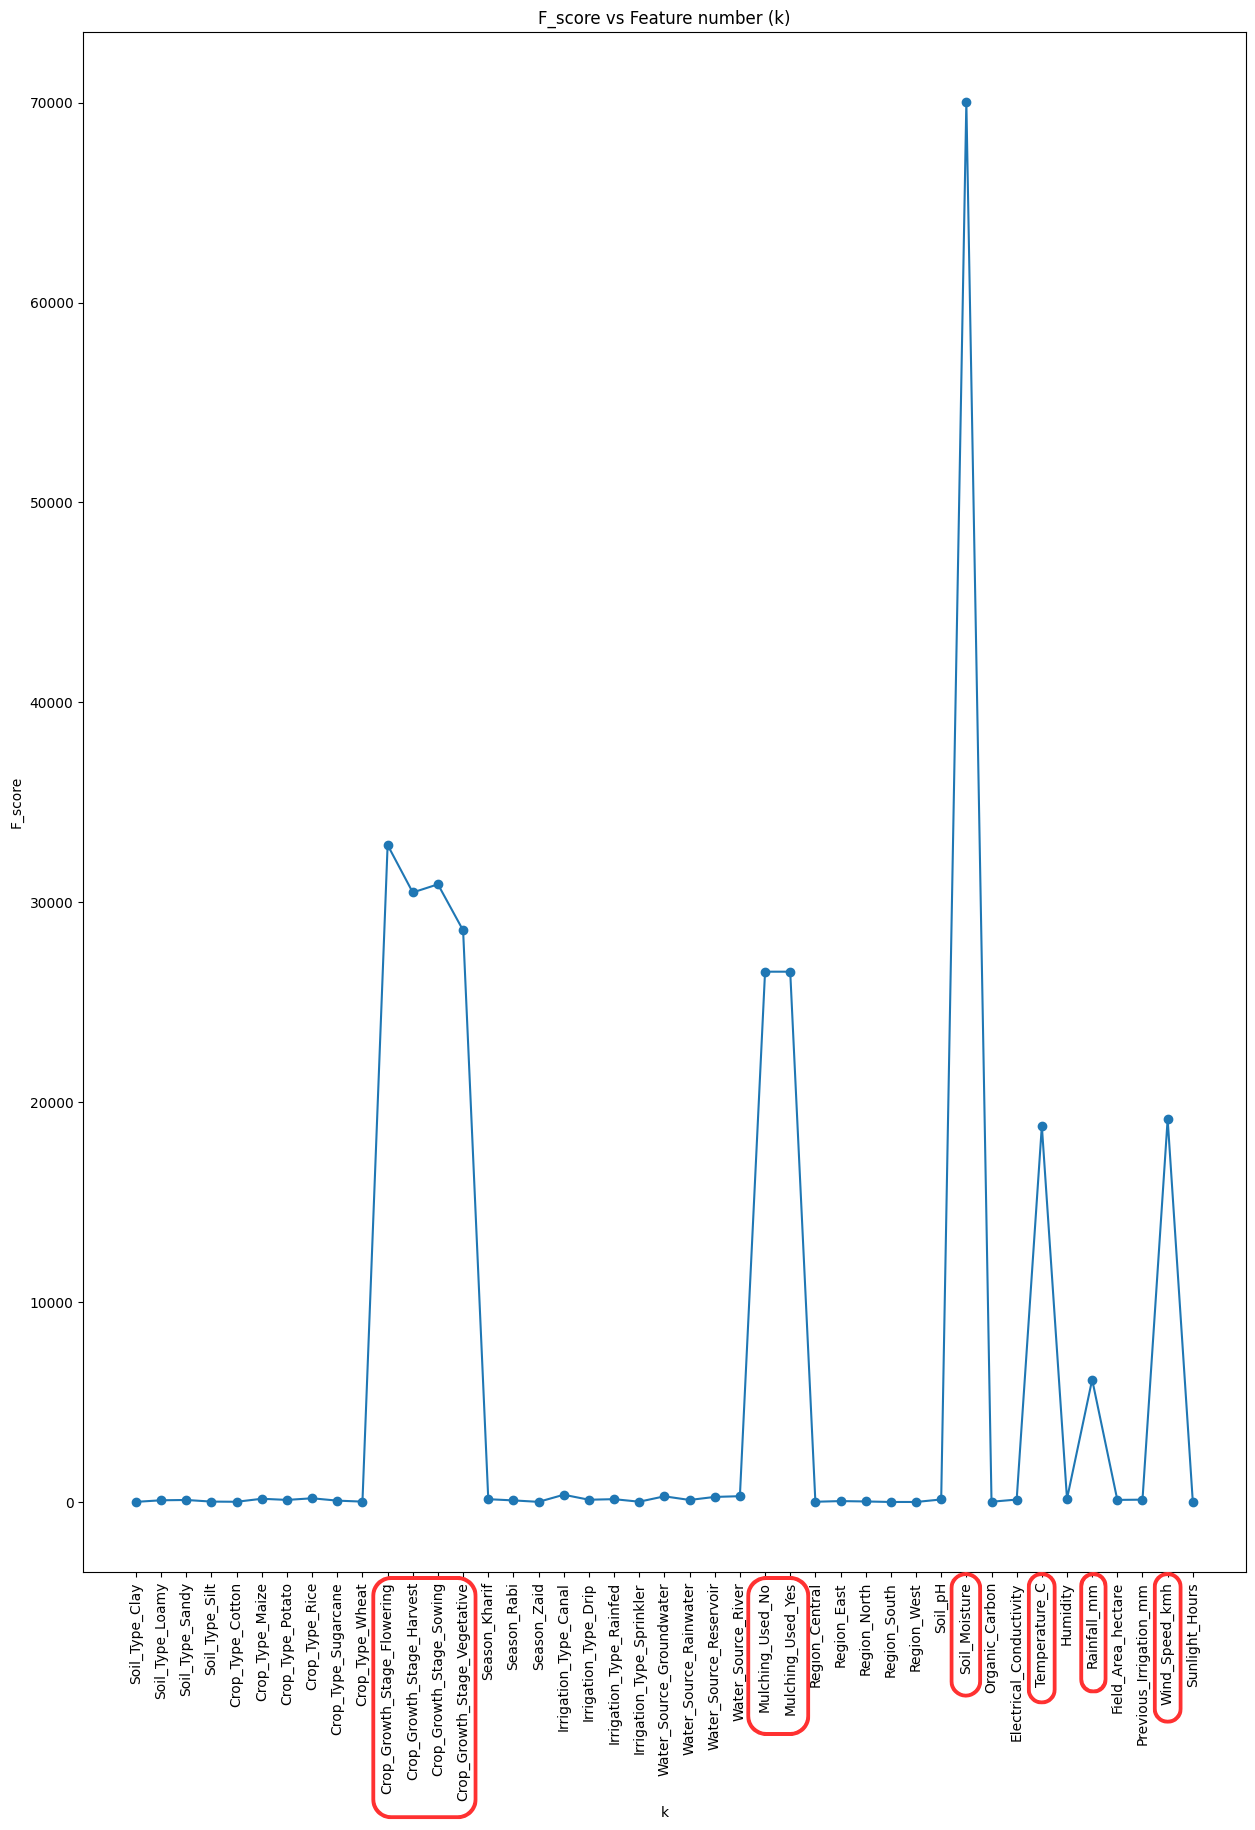
\includegraphics[width=0.5\linewidth]{lofo.png}
    \caption{The six best features are widely more relevant than the others}
    \label{fig:placeholder}
\end{figure}
\end{frame}

%=========================================================
\section{Training}
%=========================================================

\begin{frame}{Workflow and inspected models}

\paragraph{The new training set obtained has 85\% of rows of the dataset file - 15\% for testing - and the six columns divided as:\\
cols\_to\_transform = ['Soil\_Moisture','Temperature\_C','Rainfall\_mm','Wind\_Speed\_kmh']\\
cols\_to\_one\_hot\_encode = ['Crop\_Growth\_Stage','Mulching\_Used']}
\end{frame}



\begin{frame}
After first results, both \textbf{sklearn.QuantileTransformer} and \textbf{sklearn.PowerTransformer}  were tested as possible transformations for float values: QuantileTransformer  aimed to improve the uniform distribution and give robustness to outliers, but left the results almost unchanged, whereas PowerTransformer aimed to standardize the (really) different ranges of the features, and,improvement of the final score on balanced\_accuracy of +0.5\% on the train set and +0.3\% on the test set, was eventually implemented.
\\
Categorical values were encoded with One-Hot-Encoding method \textbf{sklearn.OneHotEncoder}
\\Finally, the results of such transformations were merged.
\end{frame}


\begin{frame}
As a preliminary examination, the following models were quickly valued based on accuracy:
	

	\begin{table}
	    \begin{tabular}{|l|l|>{\raggedright\arraybackslash}l|}\hline
	         \textbf{Model}&  \textbf{Score}& \textbf{Params} \\\hline
	         Gaussian N.B.&  0.772& 'var\_smoothing': 0.001\\\hline
	         Log. Regression&  0.871& 'C': 1, 'penalty': 'l2'\\\hline
 SGD Classifier& 0.865&'alpha': 0.0001, 'class\_weight': 'balanced'\\\hline
 \textbf{Decision Tree}& \textbf{0.985}&'class\_weight': None, 'max\_depth': 9\\\hline
 Perceptron& 0.835&'alpha': 0.0001, 'penalty': 'l2'\\\hline
 \textbf{AdaBoost}& \textbf{0.958}&'learning\_rate': 1.25, 'n\_estimators': 50\\\hline
 \textbf{Random Forest}& \textbf{0.985}&'class\_weight': 'balanced', 'max\_depth': 17\\\hline
 Linear SVC& 0.865&'C': 1, 'class\_weight': 'balanced'\\ \hline
	    \end{tabular}
	    \caption{Accuracy scores by different models}
	    \label{tab:placeholder}
	\end{table}
    \end{frame}
%---------------------------------------------------------

\begin{frame}{Accurate examinations}
The following examination considers all the models which have given optimal results: Decision tree classifier, Random Forest and AdaBoost. \\The final results were obtained after this model selection process and the fine tuning of their hyper-parameters.
\\For this purpose, \textbf{sklearn.GridSearchCV} was used with cross-validation split = 5 and scoring = 'balanced\_accuracy'.\end{frame}

\begin{frame}{Grid Search results}

\begin{table}
    \centering
    \begin{tabular}{|c|l|>{\raggedright\arraybackslash}p{0.5\linewidth}|}\hline
            
\textbf{Decision Tree}&\textbf{0.970}&'class\_weight': 'balanced', 'criterion': 'gini', 'max\_depth': 9, 'max\_features': None, 'min\_impurity\_decrease': 0.0, 'min\_samples_leaf': 2, 'min\_samples\_split': 5, 'splitter': 'best'\\\hline
             AdaBoost& 0.712873&'learning\_rate': 1.25, 'n\_estimators': 50\\\hline
             Random forest& 0.966256&'class\_weight': 'balanced', 'max\_depth': 10, 'max\_features': 'sqrt', 'min\_samples\_leaf': 2, 'min\_samples\_split': 3, 'n\_estimators': 20\\ \hline
    \end{tabular}
    \caption{Balanced accuracy score for selected models}
    \label{tab:placeholder}
\end{table}
\end{frame}

%---------------------------------------------------------
\begin{frame}{Results with decision tree classifier}
\centering
The balanced accuracy on train set is 96.988\%\\
The balanced accuracy on test set is 96.677\%
\begin{figure}
    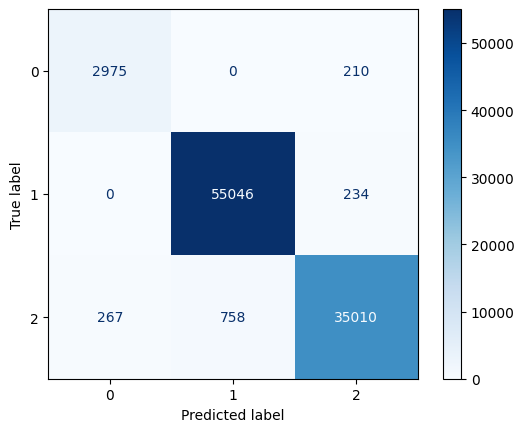
\includegraphics[width=0.7\linewidth]{confusionmatrix.png}
    \caption{Label encoder mapping \rightarrow 'High': 0, 'Low': 1, 'Medium': 2}
    \label{fig:placeholder}
\end{figure}
\end{frame}
%---------------------------------------------------------

\begin{frame}{Final comments}
Given the confusion matrix on the previous slide, the major issues to tackle for better performances could focus on the class 'Medium', giving 100\% of the misclassifications (477 with class 'High', 992 with class 'Low'), as well as implementing more regularization techniques (e.g. rounding the numerical features, optimizing other model hyper-parameters).
\end{frame}

%=========================================================
\begin{frame}{Final Remarks}
\centering
\Large Overall, the results were optimal for the task and captures the underlying data patterns correctly.

\vfill
\Huge \textbf{Thanks for your attention}
\end{frame}%=========================================================
\end{document}